Casos de uso todas las funciones del engine y diseñarlo para que la infra sea a través de consola de comandos (preparando para que luego debido a la comunicación rpc devolver los datos sea muy complicado si lo dividimos en otro comando y decidimos absorver este dominio)

El sistema está pensado para que el programa a ejecutar sea de libre decisión del cliente. pero vamos a aprovechar la oportunidad para crear un programa de control y profundizar tanto en el uso del lenguaje como en los conocimientos relacionados con este master. En concreto el control automático. Uno do los programas que podrá ejecutar será un control PID.



\begin{figure}[H]
    \centering
    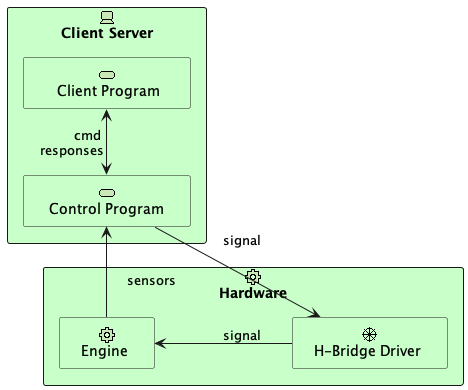
\includegraphics[height=0.3\textheight]{./part/Proyecto_ejecutivo/memoria_descriptiva/descripcionDelProyecto/control/uml/controlConcept}
    \caption[Diagrama componentes]{}\label{fig:controlConcept}
\end{figure}

\subparagraph{Dominio}

\begin{figure}[H]
    \centering
    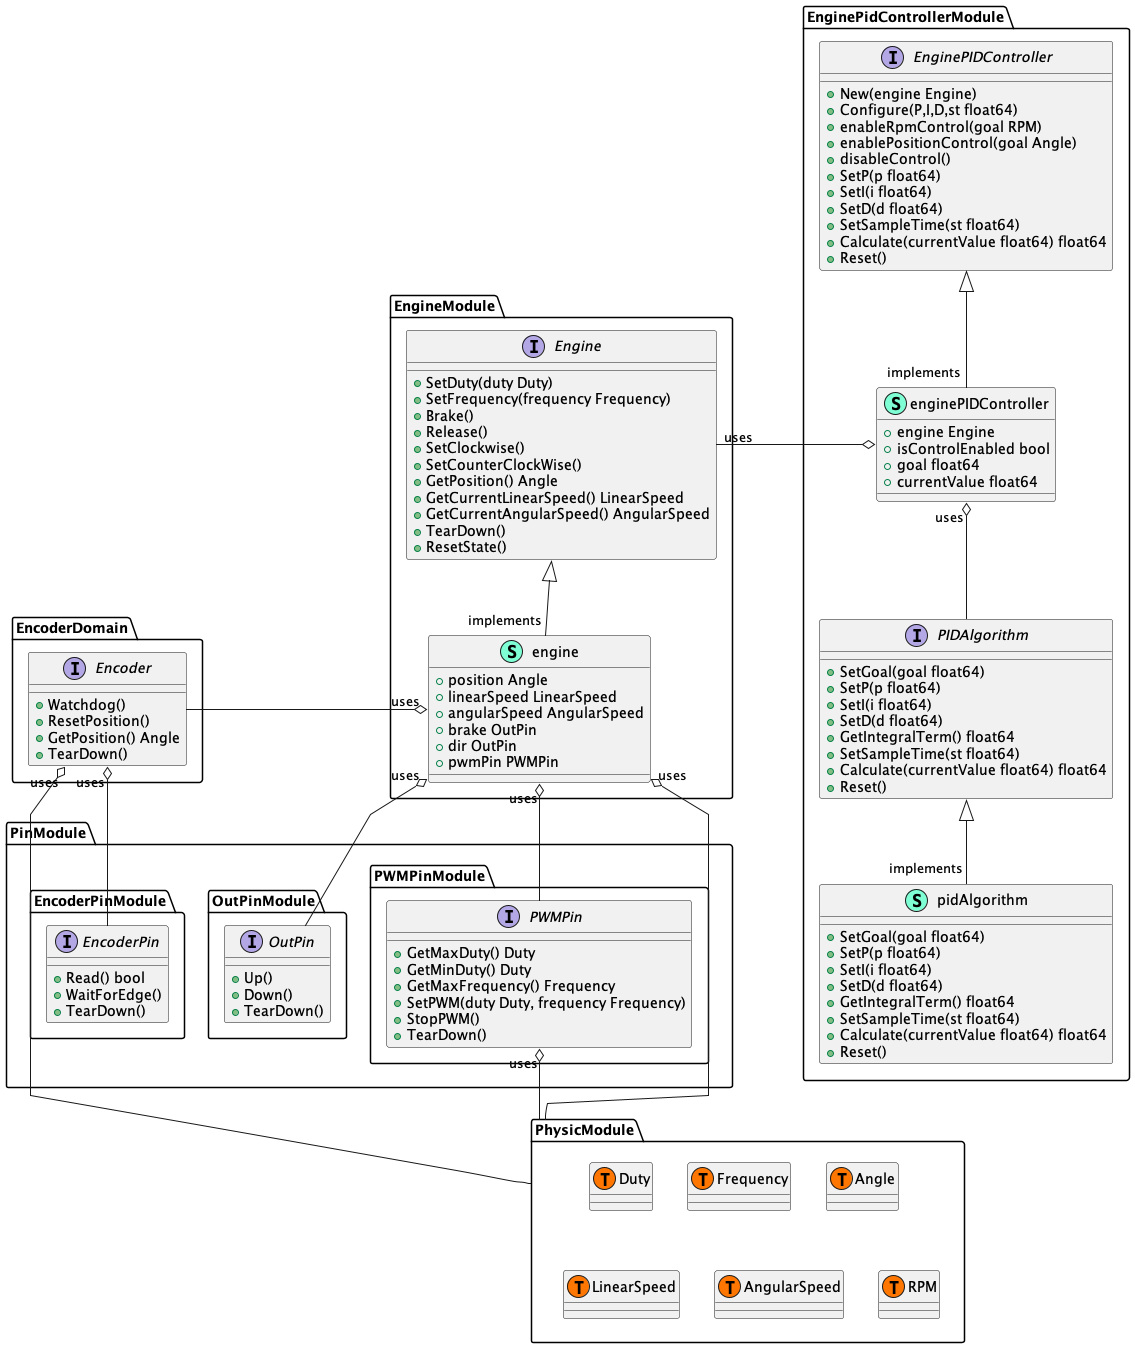
\includegraphics[height=0.4\textheight]{./part/Proyecto_ejecutivo/memoria_descriptiva/descripcionDelProyecto/control/uml/controlDomain}
    \caption[Diagrama de objetos de dominio]{}\label{fig:controlDomain}
\end{figure}

\begin{itemize}
    \item PhysicModule: contendrá todas las variables físicas, son interfaces de int y floats que usaremos para garantizar la congruencia en las operaciones. Aunque los tipos sean float hay variables que no pueden operar entre sí sin atender a su realidad física, es decir sus unidades.
    \item PinModule: para abstraernos del sistema donde se ejecute el código crearemos la abstracción de el hardware necesario para atender a interfaz física de un motor:
    \begin{itemize}
        \item EncoderPinModule: sabemos que vamos a necesitar un pin de entrada tipo pull de entrada y esperar a los flancos de subida que entrarán del encoder. Ya sea en los hardwares comerciales más conocidos como arduino o raspberry como cualquier otro.
        \item OutPinModule: para activar o desactivar frenos y triggers de dirección necesitaremos pin de salida
        \item PWMPinModule: para tener un control PWM necesitaremos un pin que nos permita salida pero con una frecuencia y un ciclo de trabajo.
    \end{itemize}
    \item EncoderModule: estará compuesto por dos pines de tipo Encoder para leer los pulsos y calcular si está en una dirección
    \item EngineModule: este modulo contendrá tanto la interfaz del motor como la implementación, donde haciendo uso de los pines calculará y contendrá las variables intrínsecas del motor.
    \item EnginePIDControllerModule: contendrá todo lo relativo al controlador PId. El controlador usará una instancia de Engine y una instancia de PIDAlgorithm
\end{itemize}

\subparagraph{casos de uso}

Los casos de usos actuarán sobre El objeto de dominio EnginePIDController, que en este caso al no haber base de datos ni identificadores serán ValueObjects. Particularmente en nuestro programa solo instanciaremos uno. No implementaremos un patrón singleton sobre ellos debido a que podría desearse controlar varios motores a la vez si el hardware lo permitiera.

\textbf{configure PID}

El primer paso a ejecutar antes de habilitar el control PID será sintonizarlo.

\begin{figure}[H]
    \centering
    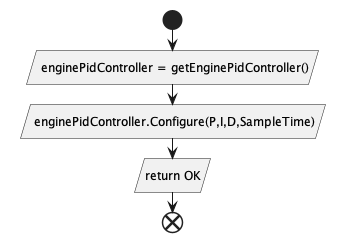
\includegraphics[height=0.2\textheight]{./part/Proyecto_ejecutivo/memoria_descriptiva/descripcionDelProyecto/control/uml/configurePID}
    \caption[Diagrama de objetos de dominio]{}\label{fig:configurePID}
\end{figure}

\textbf{enable RPM control}

Cuando se habilita el control rpm se genera una goRutine, es decir una nuevo proceso que se quedará ejecutando hasta que se ejecute el caso de uso Disable Control

\begin{figure}[H]
    \centering
    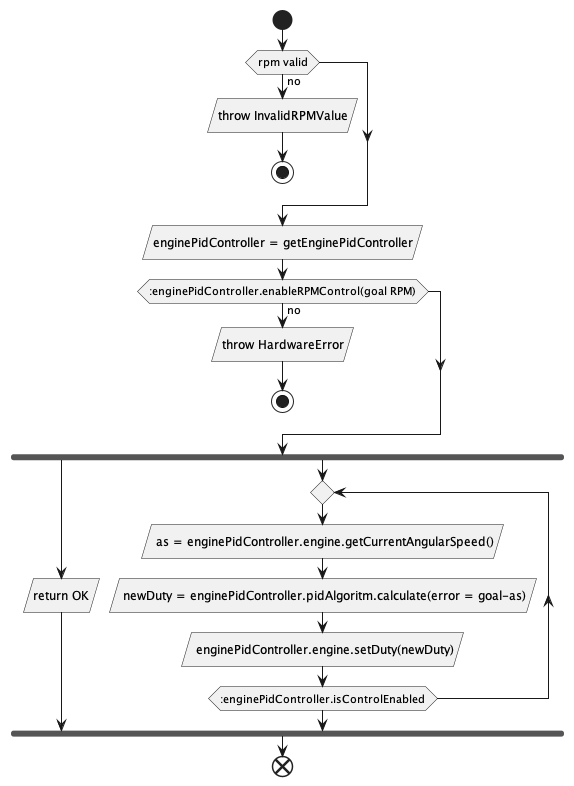
\includegraphics[height=0.4\textheight]{./part/Proyecto_ejecutivo/memoria_descriptiva/descripcionDelProyecto/control/uml/enableRPMControl}
    \caption[Diagrama de objetos de dominio]{}\label{fig:enableRMPControl}
\end{figure}

\textbf{enable Position control}

\begin{figure}[H]
    \centering
    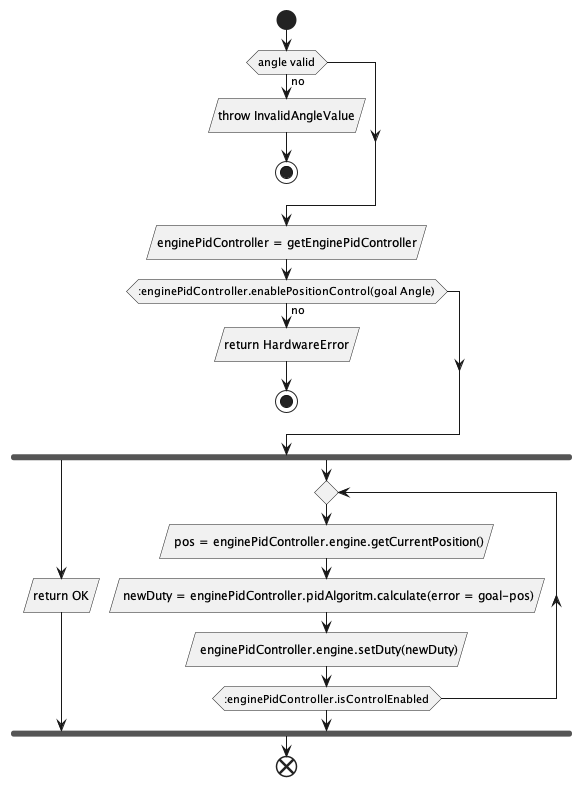
\includegraphics[height=0.4\textheight]{./part/Proyecto_ejecutivo/memoria_descriptiva/descripcionDelProyecto/control/uml/enablePositionControl}
    \caption[Diagrama de objetos de dominio]{}\label{fig:enablePositionControl}
\end{figure}

\textbf{disable control}

\begin{figure}[H]
    \centering
    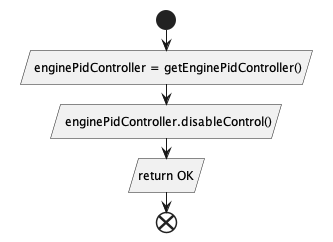
\includegraphics[height=0.2\textheight]{./part/Proyecto_ejecutivo/memoria_descriptiva/descripcionDelProyecto/control/uml/disableControl}
    \caption[Diagrama de objetos de dominio]{}\label{fig:disableControl}
\end{figure}

\subparagraph{estructura de carpetas}

En el proyecto constará de 4 carpetas principales

\tiny
\dirtree{%
    .1 Project .
        .2 Domain.
        .2 Application.
        .2 Adapter.
        .2 Bootstrap.
}
\normalsize

\textbf{Dominio}

\begin{figure}[H]
    \tiny
\dirtree{%
    .1 Domain.
        .2 Step.
            .3 StepVo.
            .3 Repository.
                .4 consoleWrite.
            .3 Services.
                .4 Executor.
        .2 Result.
            .3 ResultVo.
}
\normalsize
    \caption[Diagrama de objetos de dominio]{}\label{fig:1-controlDomain}
\end{figure}

\textbf{Aplicación}

\tiny
\dirtree{%
.1 Application.
    .2 Port.
        .3 in.
            .4 Step.
                .5 Execute.
                    .6 Command.
                    .6 UseCase.
}
\normalsize

\textbf{Adapters}

\tiny
\dirtree{%
    .1 Adapter.
        .2 in.
            .3 GRPC.
                .4 Harán uso de los useCases de aplicación cuando llegue una request RPC.
            .3 Console.
                .4 Por ejemplo si quisieramos ejecutar los casos de uso mediante terminal.
        .2 out.
            .3 console.
                .4 implementación de los repository de llamada a los servidores clientes.
}
\normalsize





